\documentclass{X:/Documents/Coding/Latex/myassignment}
\title{Topic C Assignment 3}

\begin{document}

\maketitle
\begin{enumerate}
	\item \begin{enumerate}
		\item 
		\begin{align*}
			\epsilon \frac{d^2y}{dx^2} + (\cosh x) \frac{dy}{dx} - y= 0\\
		\end{align*}
		With $y(0)=y(1)=1$
		To leading order:
		\[y = y_0 + \bigo(\epsilon)\]
		\begin{align*}
			(\cosh x)\frac{dy_{0,out}}{dx} - y_0 = 0\\
			\frac{1}{y_{0,out}}\frac{dy_{0,out}}{dx} = \sech x \\
			\log y_{0,out} = 2\arctan\left(\tanh x/2\right)\\
			\boxed{y_{0,out} = a\exp\{2\arctan\left(\tanh x/2\right)\}}
		\end{align*}


		For the boundary conditions:
		
		%answer looks like utter crap
		Let $x = x_* + \delta_1 X$, and $y = \delta_2 Y$
		\begin{align*}
			\epsilon \frac{\delta_2^2}{\delta_1^2}\frac{d^2Y}{dX^2} + (\cosh(x_* + \delta_1 X))\frac{\delta_2}{\delta_1} \frac{dY}{dX} - \delta_2 Y= 0\\
		\end{align*}
		With BCs $\delta_2 Y(0) = \delta_2 Y(1) = 1$ Hence $\delta_2 = 1$.
		\[\epsilon \frac{1}{\delta_1^2}\frac{d^2Y}{dX^2} + (\cosh(x_* + \delta_1 X))\frac1{\delta_1} \frac{dY}{dX} - Y= 0\]
		Expand the $\cosh$ term:
		\begin{align*}
			\cosh (x_*+\delta_1 X) &= \sinh(x_*)\sinh(\delta_1X)+\cosh(x_*)\cosh(\delta_1X) \\
			&=\sinh(x_*)\sum_{i=0}^\infty \frac{(\delta_1 X)^{2i+1}}{(2i+1)!}   + \cosh(x_*)\sum_{i=0}^\infty \frac{(\delta_1 X)^{2i}}{(2i)!}\\
			&= \sinh(x_*)\left(\delta_1 X\right) + \cosh(x_*) + \bigo(\epsilon^2) 
		\end{align*}
		Noting that $x^* = 0$ or $x^* =1$.
		\[\epsilon \frac{1}{\delta_1^2}\frac{d^2Y}{dX^2} + (\sinh(x_*)\left(\delta_1 X\right) + \cosh(x_*))\frac1{\delta_1} \frac{dY}{dX} - Y= 0\]
		\[\epsilon\frac{d^2Y}{dX^2} +  \delta_1^2 X \sinh(x_*)\frac{dY}{dX} + \delta_1\cosh(x_*)\frac{dY}{dX} - \delta_1^2 Y= 0\]
		Either $\delta_1 \sim \epsilon$ or $\delta_1 \sim \sqrt{\epsilon}$

		To leading order:
		Options are to neglect the $\delta$ term or the $\delta^2$ terms.
		\begin{itemize}
			\item $\delta_1^2 \sim \epsilon$
			Neglecting $\delta_1$ terms. Since $\epsilon \ll 1$, $\sqrt{\epsilon} \gg \epsilon$
			So this is not valid.

			\item $\delta_1 \sim \epsilon$, neglect the $\delta^2$ terms.
			This is reasonable.
			
		\end{itemize}
		\begin{align*}
			\frac{d^2Y_0}{dX^2} + \cosh(x_*) \frac{dY_0}{dX} = 0\\
			Y_0 = Ae^{-\cosh(x_*)X} + B	
		\end{align*}
		Since this is a negative exponential, this will not be valid as the limit
		\[\lim_{X\to-\infty} Y_0(X) = \infty\]
		And hence this holds provided $x_* =0$, giving:
		\[Y_0 = Ae^{-X} + B\]

		$Y_0(0) = 1 \implies B = 1-A$
		\[\boxed{Y_0 = Ae^{-X} + 1 -A}\]
		And applying $y(1) = 1$ gives:
		\begin{align*}
		y(1) = 1 = a\exp\{2\arctan\left(\tanh 1/2\right)\}\\
		a = \exp\{-2\arctan\left(\tanh 1/2\right)\}
		\end{align*}

		\[\boxed{Y_0 = 1 + \left(1- \exp\{-2\arctan(\tanh(1/2))\}\right)\left(e^{-X} - 1\right) }\]

		\[\boxed{y_{0} =\exp\{2\arctan\left(\tanh x/2\right) -2\arctan\left(\tanh 1/2\right) \} } \]


		Matching condition:
		\begin{align*}
			\lim_{x\to 0} y_0(x) &= \lim_{X \to \infty} Y_0(X)\\
			a\exp\{\arctan(\tanh(0))\} &= Ae^{-\infty} + 1 -A\\
			a &= 1-A\\
			A &= 1-a = 1- \exp\{-2\arctan(\tanh(1/2))\} \\
		\end{align*}

		And $y_{overlap} = a$

		Hence the composite solution is
		\begin{align*}
			y_{comp,0}(x,X) &= y_0(x) + Y_0(X) - y_{overlap}\\
			&=a\exp\{2\arctan\left(\tanh x/2\right)\} + 1 + \left(1- a\right)\left(e^{-X} - 1\right) - a\\
			y_{comp,0}(x) &=a\exp\{2\arctan\left(\tanh x/2\right)\} + 1 + \left(1- a\right)\left(e^{-x/\epsilon} - 1\right) - a\\
			%&= a\left(\exp\{2\arctan\left(\tanh x/2\right)\}  + e^{-x/\epsilon} - 1 - 1\right) +1  + e^{-x/\epsilon} - 1\\
			%&= a\left(\exp\{2\arctan\left(\tanh x/2\right)\}  + e^{-x/\epsilon} - 2\right) + e^{-x/\epsilon}\\
		\end{align*}

		\item WKB ansatz solution for
		\[\epsilon \frac{d^2y}{dx^2} + (\cosh x) \frac{dy}{dx} - y= 0\]
		\[y(x) \sim \sum_{n=0}^\infty u_n(x) \epsilon^n + e^{-F(x)/\epsilon} \sum_{n=0}^\infty v_n(x) \epsilon^{n}\] 
		Leading order:
		\begin{align*}
			y \sim u_0 + e^{-F/\epsilon} v_0\\
			y' \sim u_0' + e^{-F/\epsilon} v_0' - \frac{F'}{\epsilon} e^{-F/\epsilon}(v_0 + \epsilon v_1 + \hdots)\\
			y'' \sim u_0'' + e^{-F/\epsilon} v_0'' - 2\frac{F'}{\epsilon}e^{-F/\epsilon} v_0' + \left(\frac{F'}{\epsilon}\right)^2 e^{-F/\epsilon} \left(v_0 + \epsilon v_1 + \ldots\right) - \frac{F''}{\epsilon} e^{-F/\epsilon} v_0
		\end{align*}
		So the equation becomes:
		\begin{align*}
			\epsilon \frac{d^2y}{dx^2} + (\cosh x) \frac{dy}{dx} - y= 0\\
			\epsilon\left(u_0'' + e^{-F/\epsilon} v_0'' - 2\frac{F'}{\epsilon}e^{-F/\epsilon} v_0' + \left(\frac{F'}{\epsilon}\right)^2 e^{-F/\epsilon} \left(v_0 + \epsilon v_1 + \ldots\right) - \frac{F''}{\epsilon} e^{-F/\epsilon} v_0\right)\\
			+ \cosh x\left(u_0' + e^{-F/\epsilon} v_0' - \frac{F'}{\epsilon} e^{-F/\epsilon}(v_0 + \epsilon v_1 + \hdots)\right) - u_0 - e^{-F/\epsilon} v_0 =0\\
		\end{align*}
		Giving the system:
		\begin{align*}
			\bigo(1):0&=(\cosh x) u_0' - u_0 \\
			\bigo(e^{-F/\epsilon}/\epsilon):0&=\left(F'^2v_0  -\cosh x F' v_0\right)\\
			\bigo(e^{-F/\epsilon}): 0&=-2F'v_0' + F'^2 v_1 - F''v_0 +\cosh x v_0' -\cosh x F' v_1 - v_0\\
		\end{align*}
		\begin{align*}
			\frac{u_0'}{u_0} = \sech x\\
			\log u_0 =c+ 2\arctan\left(\tanh x/2\right)\\
			\boxed{u_0 =a\exp\left(2\arctan\left(\tanh x/2\right)\right)}
		\end{align*}
		\begin{align*}
			0&=\left(F'^2v_0  -F'v_0\cosh x  \right)\\
			0&= v_0\left(F'^2  - F'\cosh x\right)			
		\end{align*}
		For non-trivial solutions, $v_0\neq 0$ and hence
		\begin{align*}
			F'^2 - F'\cosh x = 0\\
			F' = \cosh x\\
			F = \sinh x +C
		\end{align*}
		Since the boundary layer is at $x_* = 0$, we want $e^{-F/\epsilon} = \bigo(1)$ and hence $F(0) = 0$
		\begin{align*}
			F(0) &= \sinh 0 + C\\
			&= C = 0
		\end{align*}
		Hence
		\[F = \sinh x\]
		And the third equation becomes
		\begin{align*}
			0&=-2F'v_0' + F'^2 v_1 - F''v_0 +\cosh x v_0' -\cosh x F' v_1 - v_0\\
			0&=v_1(F'^2 - F' \cosh x) -2F'v_0'- F''v_0 +\cosh x v_0' - v_0\\
			0&=-2F'v_0'- F''v_0 +\cosh x v_0' - v_0\\
			0&= -2\cosh x v_0' - \sinh x v_0  + \cosh x v_0' - v_0\\
			0&= -\cosh x v_0' - \sinh x v_0  - v_0\\
			\frac{v_0'}{v_0} &= \tanh x - \sech x\\
		\end{align*}
		Rather than directly solving that, ill just use the boundary conditions:
		\begin{align*}
			y(1) = 1 \implies u(1) = 1\\
			\implies a=\exp\{-2\arctan\left(\tanh 1/2\right)\}\\
			y(0) = 1 \implies u_0(0) + v_0 = 1\\
			v_0 = 1- a
		\end{align*}

		Hence
		\begin{align*}
			y_{WKB,0} &= u_0 + e^{-F/\epsilon} v_0\\
		\end{align*}
		\[\boxed{y_{WKB,0}=a\exp\left(2\arctan\left(\tanh x/2\right)\right)+ \exp\left(-\sinh x/\epsilon\right)(1-a) }\]
		Where
		\[a =\exp\{-2\arctan\left(\tanh 1/2\right)\}\]



		\item First rewrite the BVP in a nicer format
		\[\frac{d^2y}{dx^2} + \frac{1}{\epsilon} \left(\cosh x\frac{dy}{dx} - y\right) = 0\] 
		Figure~\ref{fig:q1} shows the comparison of the five solutions - the numerically obtained, inner, outer, composite and WKB ansatz solutions. Clearly the inner and outer solutions approach the 3 full solutions (numeric, composite, WKB) near the boundary values, and the full solutions match quite closely (with a gap forming around $x=0.2$). The value $\epsilon = 0.2$ has been chosen to show that there is a small discrepancy in the answers, particularly around this gap.
	\begin{figure}[tb]
		\centering
		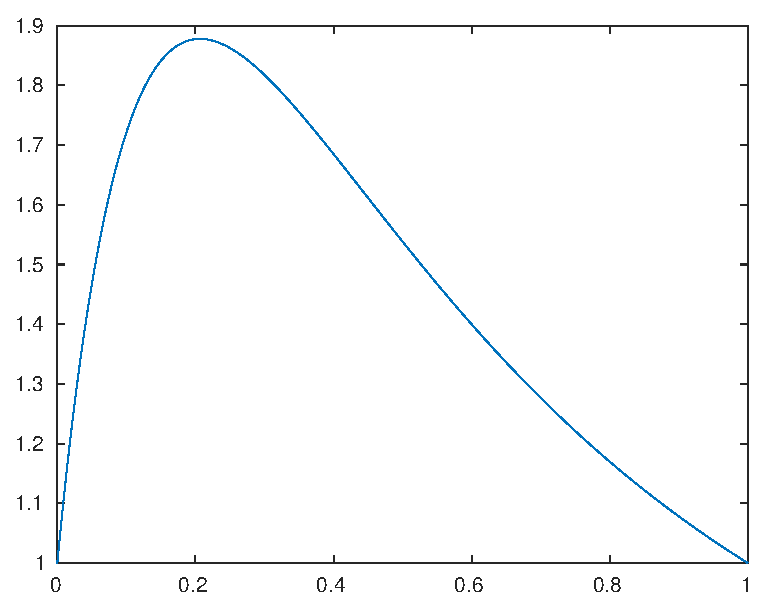
\includegraphics{TopicCA3Q1}
		\caption{Comparison of Numerical, WKB and Composite solutions for $\epsilon = 0.2$}
		\label{fig:q1}
	\end{figure}
	\end{enumerate}


	\clearpage
	\item 
	%Find leading order solutions to
	\[\epsilon \frac{d^2y}{dx^2} + x\frac{dy}{dx} + xy =0\]
	With $y(-2)=-4$ and $y(2) =2$, $\epsilon \to 0$ over $-2\leq x \leq 2$. There is an internal boundary layer shown via the numerical solution, in figure~\ref{fig:q2}

	The right outer solution $y_R$ with $y_R(2) = 2$ to leading order:
	\begin{align*}
	xy_{R0}' + xy_{R0} = 0\\
	y_{R0}' + y_{R0} = 0\\
	y_{R0} = Ae^{-x}
	\end{align*}
	And applying the boundary condition:
	\begin{align*}
		y_{R0}(2) = Ae^{-2} = 2\\
		A = 2e^2
	\end{align*}

	\[\boxed{y_{R0} = 2e^2e^{-x} } \]
	
	The left outer solution $y_L$ with $y_L(-2) =-4$
	\begin{align*}
	y_{L0} = Be^{-x}\\
	y_{L0}(-2) = Be^{-2} = -4\\
	B = -4e^{-2}
	\end{align*}
	Hence
	\[\boxed{y_{L0} = -4e^{-2}e^{-x} } \]

	For the inner solution $x = x_* + \delta_1 X$, and $y = \delta_2 Y$. Since the boundary conditions don't include $\epsilon$, $\delta_2 =1$.
	\begin{align*}
		\epsilon \frac{d^2y}{dx^2} + x\frac{dy}{dx} + xy =0\\
		\epsilon \frac{1}{\delta_1^2}\frac{d^2Y}{dX^2} + (x^* + \delta_1X)\frac{1}{\delta_1}\frac{dY}{dX} + (x^* +\delta_1 X)Y =0\\
		\epsilon \frac{d^2Y}{dX^2} + \delta_1 (x^* + \delta_1 X)\frac{dY}{dX} + \delta_1^2 (x^* + \delta_1X)Y = 0\\
		\epsilon \frac{d^2Y}{dX^2} + \delta_1 x^*\frac{dY}{dX} + \delta_1^2 X\frac{dY}{dX} + \delta_1^2 x^*Y+ \delta_1^{3}XY = 0\\
		\epsilon \frac{d^2Y}{dX^2} + \delta_1 x^*\frac{dY}{dX} + \delta_1^2\left( X\frac{dY}{dX} + x^*Y\right)+ \delta_1^{3}XY = 0\\
	\end{align*}
	% Taking the perturbation series:
	% \[Y = Y_0 + \epsilon Y_1 + \epsilon^2 Y_2\]
	% \begin{align*}
	% 	&\epsilon \frac{d^2(Y_0 + \epsilon Y_1 + \epsilon^2 Y_2 +\hdots)}{dX^2} + \delta_1 x^*\frac{d(Y_0 + \epsilon Y_1 + \epsilon^2 Y_2 + \hdots)}{dX} \\
	% 	&+ \delta_1^2\left( X\frac{d(Y_0 + \epsilon Y_1 + \epsilon^2 Y_2 + \hdots)}{dX} + x^*(Y_0 + \epsilon Y_1 + \epsilon^2 Y_2 + \hdots)\right)\\
	% 	&+ \delta_1^{3}X(Y_0 + \epsilon Y_1 + \epsilon^2 Y_2 + \hdots) = 0\\
	% \end{align*}
	% %%%%ALl this is wrong
	Balances:
	\begin{itemize}
		\item $\epsilon \frac{d^2Y}{dX^2} \sim -\delta_1 x^*\frac{dY}{dX}$ Hence $\delta_1 \sim \epsilon$, this is reasonable since the rejected terms will be $\bigo(\epsilon^2)$ and $\bigo(\epsilon^3)$ both of which are negligible.
		\item $\epsilon \frac{d^2Y}{dX^2} \sim - \delta_1^2\left( X\frac{dY}{dX} + x^*Y\right) $ giving $\delta \sim \sqrt{\epsilon}$ neglecting terms of order $\epsilon^{1/2}$ and $\epsilon^{3/2}$. But $\epsilon^{1/2}\gg \epsilon$ so this is a contradiction. 
		\item $\epsilon \frac{d^2Y}{dX^2} \sim - \delta_1^{3}XY $ with $\delta_1 \sim \epsilon^{1/3}$, meaning we have neglected the $\epsilon^{1/2}$ and $\epsilon^{1/3}$ terms in favour of $\epsilon$. This is a contradiction since $\epsilon^{1/3} \gg \epsilon$
		\item $\delta_1 x^*\frac{dY}{dX} + \delta_1^2\left( X\frac{dY}{dX} + x^*Y\right)\sim - \delta_1^{3}XY$. Implying $\delta_1 \sim 1$. For $x^* = 0$ this is precisely the outer region.
	\end{itemize}
	Hence take $\delta_1 = \epsilon$

	To leading order:
	\begin{align*}
	\frac{d^2Y_0}{dX^2} = - x^*\frac{dY_0}{dX}\\
	V' = -x^* V\\
	\implies V = ae^{-x^* X}\\
	\implies Y_0 =a_0 e^{-x^* X} +b
	\end{align*}
	Assuming $x^* \neq 0$.

	We have to match this to the left and right solutions
	Conditions
	\[\lim_{x\to x^*} y_{R0}(x) = \lim_{X\to\infty} Y_0(X), \quad \& \quad \lim_{x\to x^*} y_{L0}(x) = \lim_{X\to-\infty} Y_0(X)\]
	For non-zero $x^*$ this gives:

	\begin{align*}
		\lim_{x\to x^*} y_{R0}(x)&=\lim_{X\to \infty} Y_0(X)\\
		\lim_{x\to x^*} 2e^2e^{-x} &= \lim_{X\to \infty} a_0 e^{-x^* X} +b\\
		2e^2e^{-x_*} &= \lim_{X\to \infty} a_0 e^{-x^* \infty} +b
	\end{align*}
	For the right, and for the left:
	\begin{align*}
		\lim_{x\to x^*} y_{L0}&=\lim_{X\to -\infty} Y_0(X) \\
		\lim_{x\to x^*} -4e^{-2}e^{-x} &= \lim_{X\to -\infty} a_0 e^{-x^* X} +b\\
		-4e^{-2}e^{-x_*} &= \lim_{X\to -\infty} a_0 e^{x^* \infty} +b
	\end{align*}
	For both of these to hold, we would require $x^* = 0$ (which we assumed wasn't true). So take $x^* = 0$ and resolve the DE:
	\[\epsilon \frac{d^2Y}{dX^2} + \delta_1^2 X \frac{dY}{dX} + \delta_1^3 Xy = 0 \]
	with $\delta_1 \sim \epsilon$
	\begin{align*}
		\frac{d^2Y_0}{dX^2} +  X \frac{dY_0}{dX} &= 0 \\
		V' &= -XV\\
		V &= ae^{-X^2}\\
		Y_0 &= \int V dX= \int ae^{-X^2} dX\\
		&= a \mathrm{erf}(\frac{X}{\sqrt2}) + b
	\end{align*}
	%it may be a slightly different form
	Matching conditions:
	\begin{align*}
		\lim_{x\to 0} y_{R0}(x)&=\lim_{X\to \infty} Y_0(X)\\
		2e^2e^{0} &= a\mathrm{erf}(inf) + b\\
		2e^2 &= a + b
	\end{align*}
	\begin{align*}
		\lim_{x\to 0} y_{L0}&=\lim_{X\to -\infty} Y_0(X) \\
		-4e^{-2} &=  a\mathrm{erf}(-inf) + b\\
		-4e^{-2} &=  -a + b
	\end{align*}
	\begin{align*}
		 a + b &= 2e^2\\
		-a + b &= -4e^{-2}\\
		2b &= 2e^{2} - 4e^{-2}\\
		b &= e^{2} - 2e^{-2}\\
		a + e^{2} - 2e^{-2} &= 2e^{2}\\
		a &= e^{2} + 2e^{-2}
	\end{align*}

	\[\boxed{Y_0(X) = \left(e^{2} + 2e^{-2}\right)\mathrm{erf}(\frac{X}{\sqrt{2}}) + e^{2} - 2e^{-2}}\]
	Figure~\ref{fig:q2} shows the comparison of solutions. The outer solutions clearly match the boundary conditions, while the inner solution does not obviously match the inner region. 

	\begin{figure}[tb]
		\centering
		\label{fig:q2}
		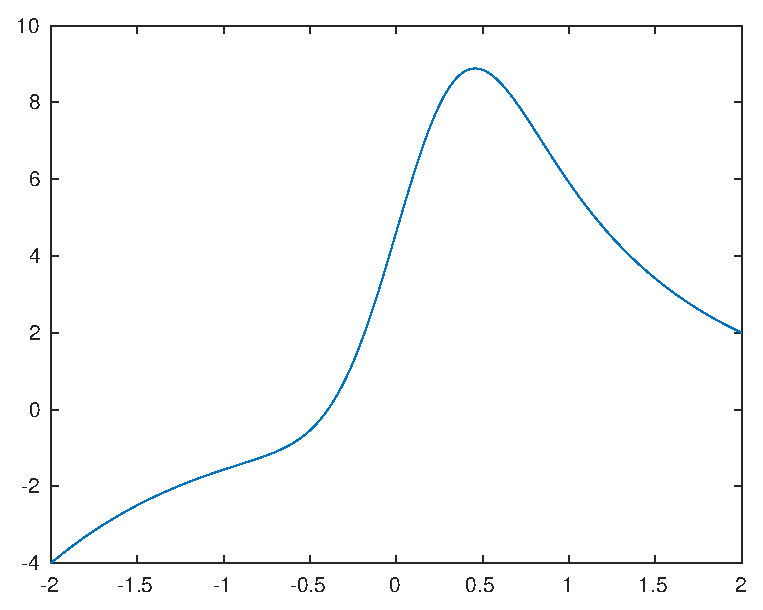
\includegraphics{TopicCA3Q2}
		\caption{Plot of the internal boundary layer problem for $\epsilon = 0.1$. The left, and right outer solutions, and the inner solution are plotted.}
	\end{figure}
\end{enumerate}

\section*{Matlab Code}
\lstinputlisting{AppTopicCA3.m}

\clearpage
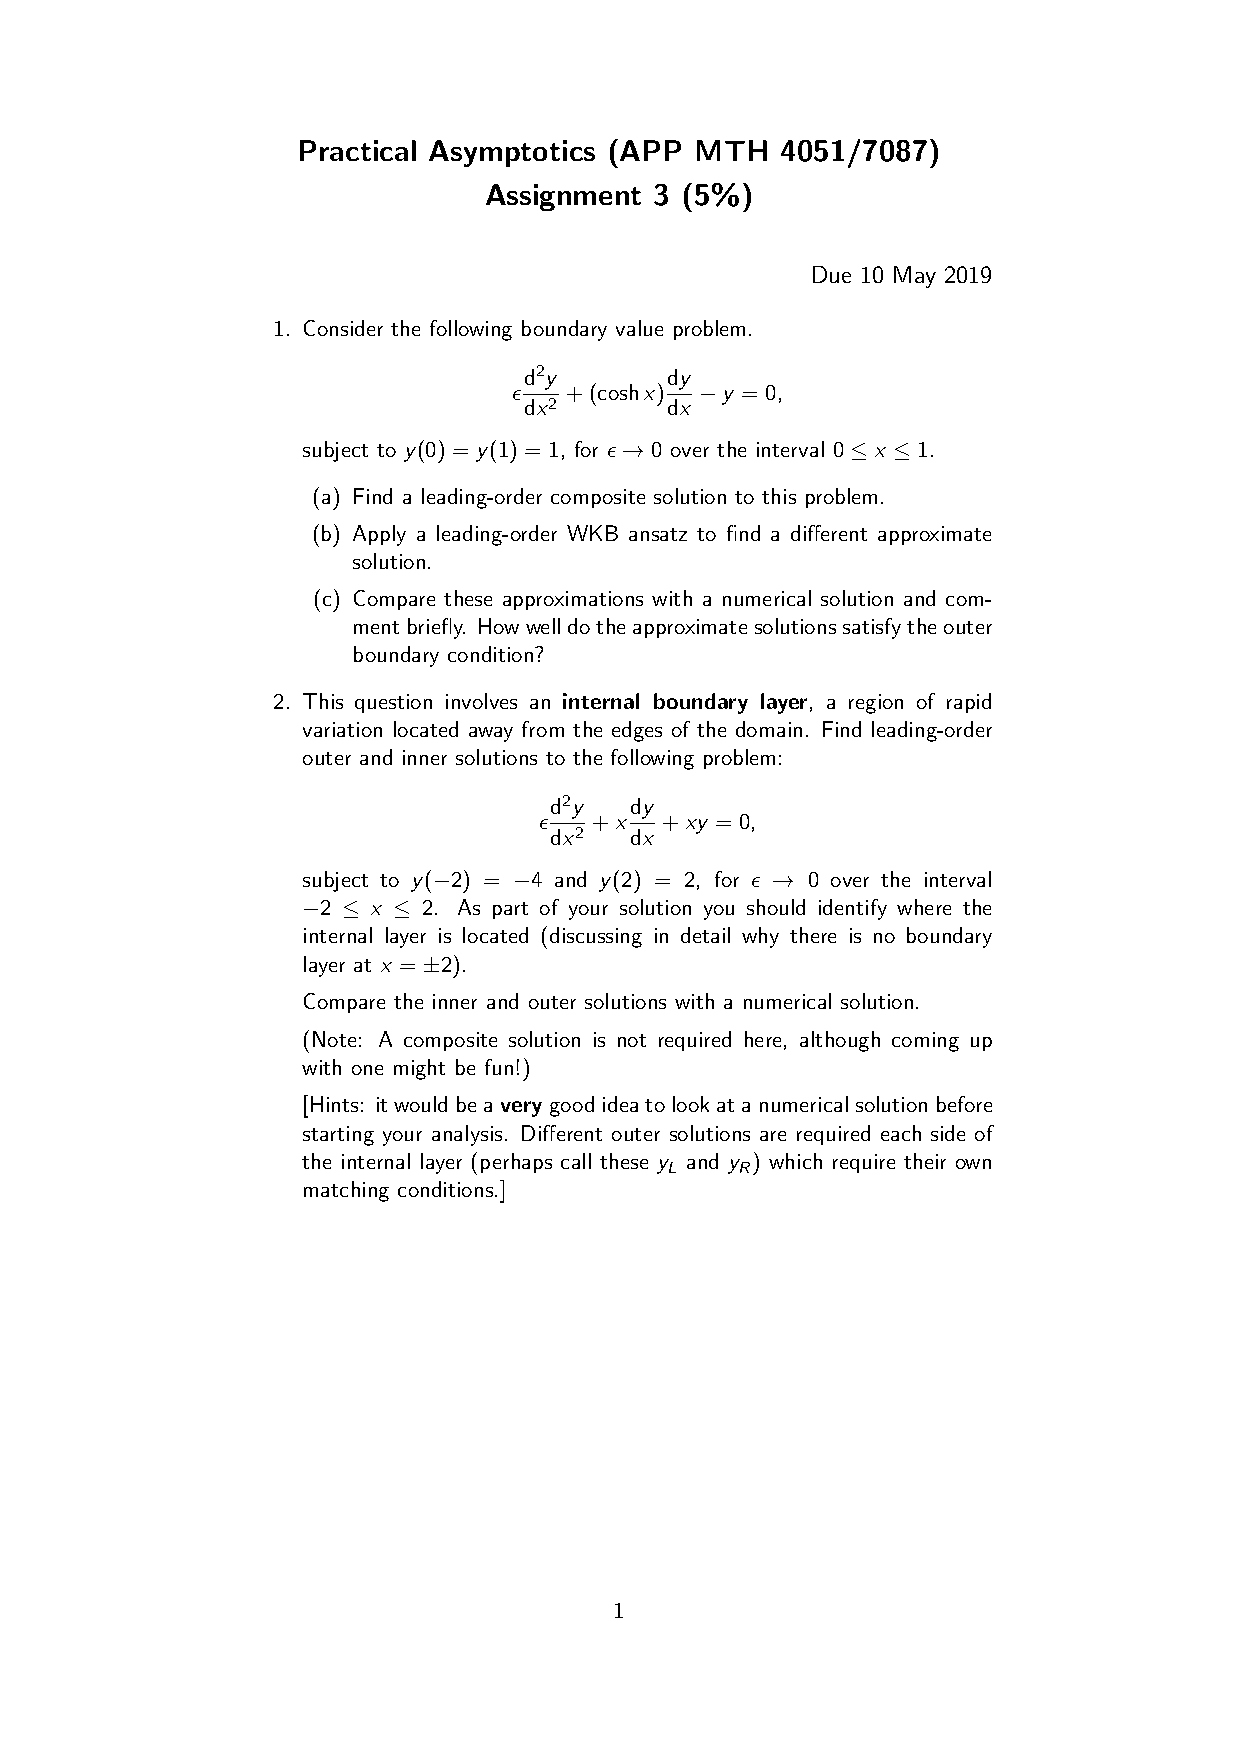
\includepdf[pages=1-]{PA_2019_A3.pdf}




\end{document}